%----------------------------------------------------------------------------------------
%	Introducción
%----------------------------------------------------------------------------------------

\newpage
\clearpage{\pagestyle{empty}\cleardoublepage}
%\doublespacing
\newpage

\pagestyle{myportland}
\pagenumbering{arabic}

\chapter*{\centering \large Introducción} 
\addcontentsline{toc}{chapter}{Introducción} % si queremos que aparezca en el índice
\markboth{Introduction}{Introducción} % encabezado

\thispagestyle{myportland}

 El potencial acuícola del Perú debido a sus lagos y lagunas a lo largo de la sierra es alto. Sin embargo, la producción se concentra en el departamento de Puno, se procesa de forma manual y carece de automatización de grado alimenticio. El presente trabajo parte de un diseño conceptual previo que se elabora en sus aspectos técnicos de ingeniería siguiendo normas internacionales de diseño. El sistema (Figura \ref{fig:total con operarios}) se diseña acorde a una lista de requerimientos tomada en cuenta en el diseño conceptual. Dicho sistema es una solución de semi-automatización que brinda una opción a los altos costos de las máquinas comerciales que no están diseñadas para las condiciones peruanas. La propuesta del sistema permite disminuir el proceso de clasificación y conteo de 7 a 1 día y con un trabajador menos. En las siguientes líneas se introducen los capítulos del trabajo.
 
 En el capítulo 1 se revisan los antecedentes, la problemática a la que se presenta una solución, el alcance del proyecto, los objetivos y, la metodología normativa y de desarrollo ingenieril. En el capítulo 2 se elabora el diseño mecatrónico integral donde se presentan los subsistemas del proyecto, se brinda una arquitectura de hardware a seguir para los componentes eléctricos y electrónicos, además de un análisis técnico de los materiales para brindar una máquina de grado alimenticio. Además se presenta los programas y algoritmos codificados, la lista de los planos y se presenta de manera breve el sistema de flotación. En el capítulo 3 se diseña el subsistema de recepción, distribución y traslado de truchas que desarrolla la forma en cómo se recibe a la trucha, se traslada mediante caudal de agua y se distribuye mediante un mecanismo. En el capítulo 4 se diseña el subsistema de procesamiento de imágenes, la selección de cámaras y sensor infrarrojo junto con su posicionamiento, se listan los algoritmos posibles y se escogen algunos, se recopila una base de datos de imágenes y se prepara para los algoritmos seleccionados. En el capítulo 5 se diseña el subsistema de control e interacción con el usuario se selecciona el microprocesador, sus indicadores y el frontend de interfaz del usuario. Además, se presenta los lazos de control de los mecanismos dentro del subsistema. En el capítulo 6 se diseña el subsistema de suministro de energía, la selección de convertidores de voltaje de conmutación y fuentes de alimentación acorde a las directivas del capítulo 2. En el capítulo 7 se presenta pruebas y resultados de los algoritmos de clasificación y conteo que se separan en cuatro etapas. Además, se realiza un análisis estructural. En el capítulo 8 se estima los costos del sistema y se obtiene un costo de fabricar y ensamblar una máquina de aproximadamente \$4900, el cuál no es comparable con los precios comerciales. Finalmente se presenta las conclusiones y recomendaciones.

%Considera los siguientes puntos:
%\begin{enumerate}
%	\item Desarrolle un único párrafo (200 a 300 palabras)
%	\item Escriba en tiempo verbal presente
%	\item El resumen debe contener información sobre:
%	\begin{itemize}
%		\item	- La justificación de la investigación
%		\item	- Los objetivos o hipótesis
%		\item	- La teoría o supuestos teóricos o metodológicos en la que se sustenta
%		\item	- El método o procedimiento realizado (de ser necesario)
%		\item	- Los resultados (de ser necesario)
%		\item	- La conclusión principal
%	\end{itemize}
%\end{enumerate}


\begin{myfigure}[H]
	\centering
	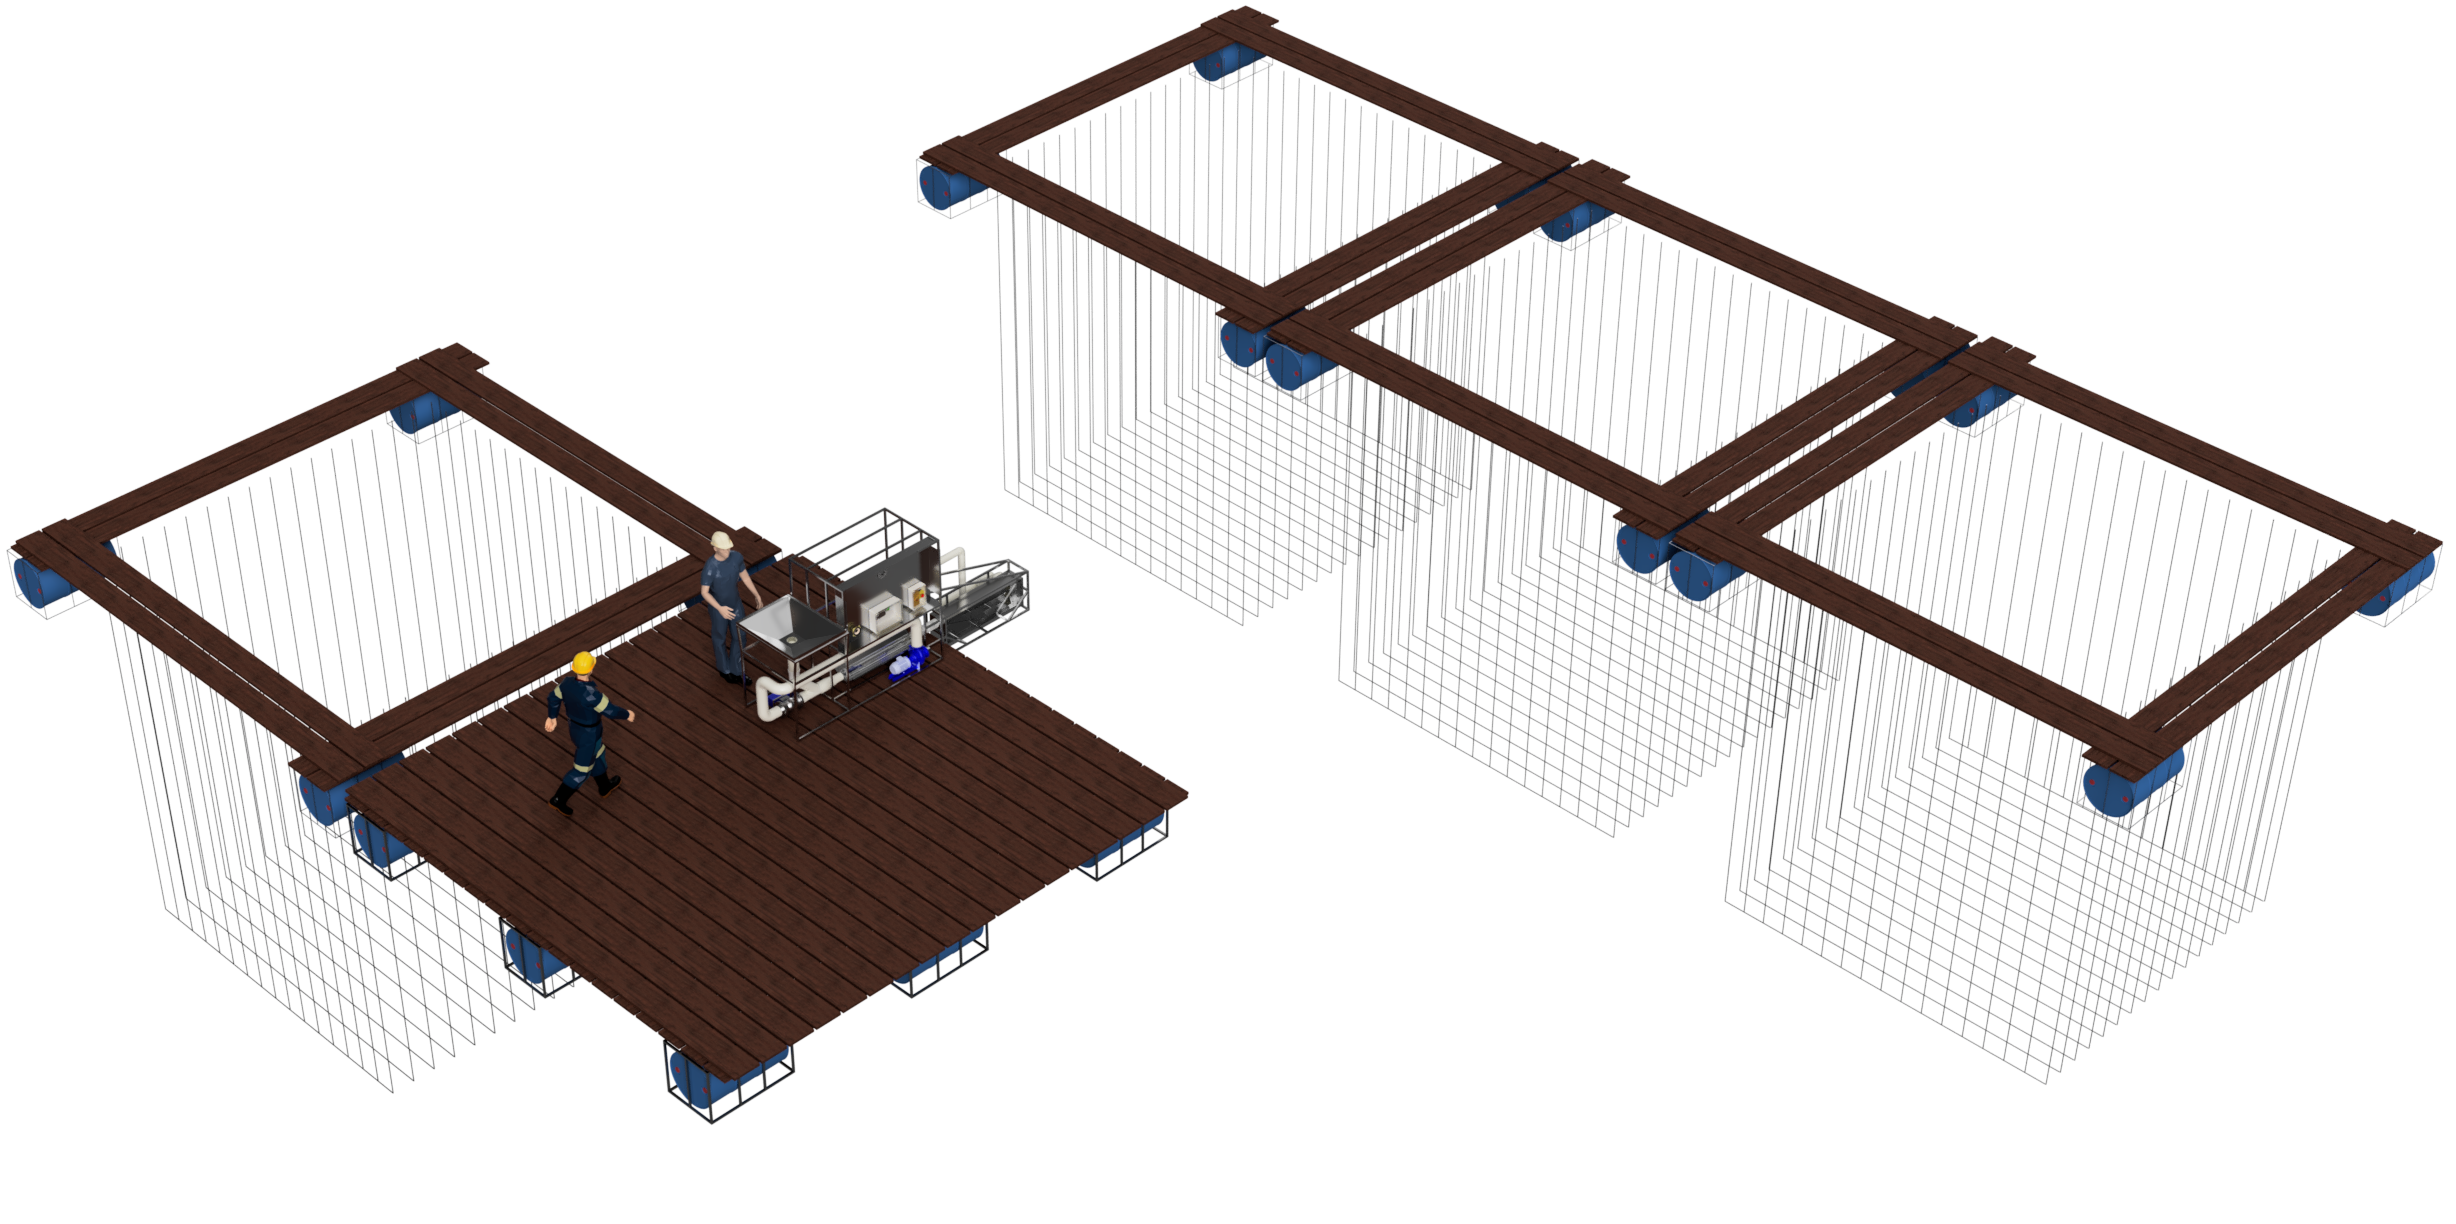
\includegraphics[width=1\textwidth]{total con operarios.png}
	\caption{Sistema propuesto en el presente trabajo.}
	\begin{myflushcenter}
		Fuente: Elaboración propia.
	\end{myflushcenter}
	\label{fig:total con operarios}
\end{myfigure}